%!TEX root = ../main.tex
%%%%%%%%%%%%%%%%%%%%%%%%%%%%%%%%%%
% Links:
%
% Difficulty:
% Companies: 
%%%%%%%%%%%%%%%%%%%%%%%%%%%%%%%%%%


%\begin{figure}
%	\centering
%	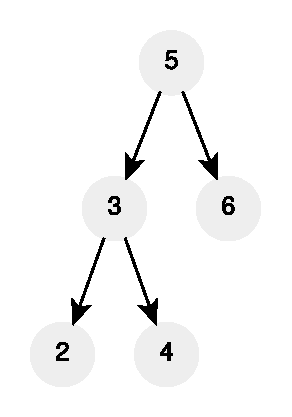
\includegraphics[width=\textwidth]{sources/max_triplet/images/example1}
%	\caption[Sample short cpation]{Sample Caption}.
%	\label{fig:max_triplet:example1}
%\end{figure}

\chapter{Max triplet sum }
\label{ch:max_triplet}
\section*{Introduction}

\section{Problem statement}
\begin{exercise}
\label{example:max_triplet:exercice1}
Problem Description

Given an array A containing N integers.

You need to find the maximum sum of triplet ( Ai + Aj + Ak ) such that 0 <= i < j < k < N and Ai < Aj < Ak.

If no such triplet exist return 0.



Problem Constraints
3 <= N <= 105.

1 <= A[i] <= 108.



Input Format
First argument is an integer array A.



Output Format
Return a single integer denoting the maximum sum of triplet as described in the question.



Example Input
Input 1:

 A = [2, 5, 3, 1, 4, 9]
Input 2:

 A = [1, 2, 3]


Example Output
Output 1:

 16
Output 2:

 6


Example Explanation
Explanation 1:

 All possible triplets are:-
    2 3 4 => sum = 9
    2 5 9 => sum = 16
    2 3 9 => sum = 14
    3 4 9 => sum = 16
    1 4 9 => sum = 14
  Maximum sum = 16
Explanation 2:

 All possible triplets are:-
    1 2 3 => sum = 6
 Maximum sum = 6
	%example1
	\begin{example}
		\label{example:max_triplet:example1}
		\hfill \
	}
		
	\end{example}

	%example2
	\begin{example}
		\label{example:max_triplet:example2}
		\hfill \
		
	\end{example}

	\begin{example}
		\hfill \
	
	\label{ex:max_triplet:example1}
	\end{example}

	\begin{example}
		\hfill \

	\label{ex:max_triplet:example2}	
	\end{example}
\end{exercise}

\section{Clarification Questions}

\begin{QandA}
	\item 
	\begin{answered}
		\textit{}
	\end{answered}
	
\end{QandA}

\section{Discussion}
\label{max_triplet:sec:discussion}


\subsection{Brute-force}
\label{max_triplet:sec:bruteforce}

\begin{minipage}{\linewidth}
	\lstinputlisting[language=c++, caption={Sample Caption},label=list:max_triplet]{sources/max_triplet/max_triplet_solution1.cpp}
\end{minipage}

